\chapter{Optisches Filtern}
Der letzte Versuch heißt optisches Filtern. Mithilfe unterschiedlicher Aufbauten werden die Grundideen der Abbe'schen Abbildungstheorie vermittelt. \\
Der Physiker Ernst Abbe entschlüsselte  um 1870 geradezu akribisch die Bildentstehung im Mikroskop. 
Im Jahr 1867 schlug Ernst Carl Abbe eine Theorie vor, die die Grenzen des Auflösungsvermögens von optischen Systemen und deren Verbindung mit der Wellenlänge verdeutlicht.
Durch die dadurch gewonnenen Erkenntnisse gelangen Ernst Abbe bahnbrechende Verbesserungen im Bereich der mikroskopischen Optik. 
Somit war es möglich Objektive zu berechnen, bei denen die relevanten Abbildungsfehler weitgehend korrigiert sind. Allerdings entstehen beim Bau dieser Objektive zunächst unüberwindliche Schwierigkeiten, da die hierzu notwendigen optischen Gläser zu jener Zeit einfach nicht verfügbar sind. Es ist dann der Glaschemiker Otto Schott, dem es gelingt Gläser mit den benötigten optischen Eigenschaften herzustellen.
Die Abbe'sche Abbildungstheorie geht davon aus, dass jedes Objekt Beugungseffekte hervorruft. Somit wird die Bildinformation des Objektes auf die Beugungsmaxima aufgeteilt.
	
Es können also mehr Informationen aufgenommen werden, wenn mehr Maxima für die Bildgebung genutzt werden.
Allerdings ist natürlich die Öffnung eines Objektives nicht unendlich groß, sodass nicht alle Maxima eingefangen werden können.
Für eine minimale Strukturinformation müssen mindestens die Maxima der nullten und der ersten Ordnung erfasst werden.
Ist die Objektivöffnung zu klein, gelangen die Maxima der ersten Ordnung nicht mehr ins Objektiv und es kann kein Bild entstehen.



\section{Fragen und Aufgaben}
\begin{itemize}
	\item 1. Wie lautet die Abbildungsgleichung für Linsen und was bedeuten die einzelnen Größen?\\
	$\frac{1}{b}+\frac{1}{g}=\frac{1}{f}$ falls $d \ll r_1, r_2$\\
	g= Gegenstandsweite \\
	b= Bildweite\\
	f= Brennweite\\ \\
	\item 2. Tragen Sie in die untenstehende Abb. of.1 die entsprechenden Grössen der Abbildungsgleichung	ein und konstruieren Sie das Bild des Gegenstands G. Vergleichen Sie die konstruierten Werte für Bildgrösse und Bildweite mit den berechneten.\\
	
		\begin{figure}[h]
		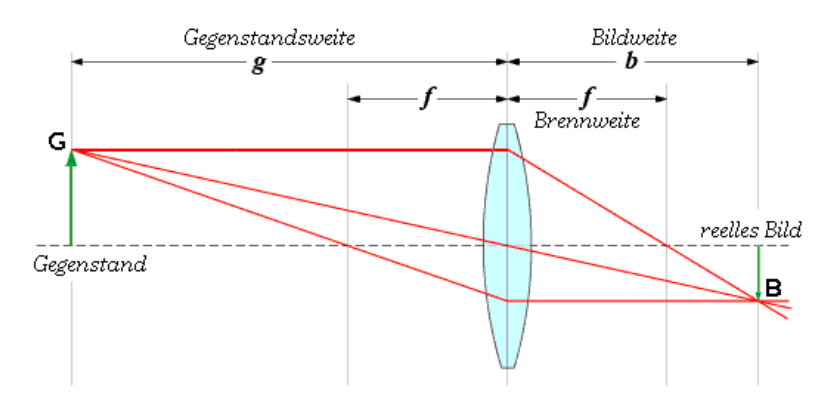
\includegraphics[width=1\textwidth]{abbildungsgl}
		\caption{Konstruktion der Größen der Abbildungsgleichung} 
	\end{figure}
Größen in Skizze: f= 3,1 cm , g= 8,5 cm , G= 1,9 cm 
	
	gemessene Werte: \\b = 4,9 cm\\B= 1,1cm
	\\\\
	berechnete Werte: \\b= $\Big(\dfrac{1}{f} - \dfrac{1}{g}\Big)^{-1} = 4,9 cm$
\\	$B = \dfrac{\Big(\dfrac{1}{f} - \dfrac{1}{g}\Big)^{-1}-f}{f}G= 1,1 cm   $

	\item 3. Sie benutzen im Versuch einen Laserstrahl, dessen enges Ausgangsstrahlbündel (näherungsweise)
	zu einem breiteren Parallelstrahl aufgeweitet wird (siehe Abb. of.2). Dazu sollen zwei
	Linsen L1 und L2 verwendet werden. L1 habe $f_1$ = 10mm und die Aufweitung soll 8-fach sein.
	Es stehen für L2 Linsen mit 80, 100 und 200mm zur Verfügung. Welche würden Sie wählen?
	Wie groß müssen die Linsendurchmesser mindestens sein?\\
	Vergrößerung = $\dfrac{f_1}{f_2}$\\
	$\Rightarrow f_2=8 \cdot 10 \text{ mm}=80 \text{ mm}$\\
	Angenommene Eingangsstrahlbreite: 5mm\\ $\Rightarrow$ Für zweiten Linsendurchmesser $d_2$ muss gelten: \\
	$d_2 \geq V \cdot d_1= 40 \text{ mm}$
\\Wenn man davon ausgeht, dass die Eingangsstrahlbreite 5 mm beträgt, wäre es sinnvoll die 80mm-Linse mit mindestens 40mm als $d_2$ zu benutzen. \\\\\\\\\\\\\\\\\\\\\\\\
	\item 4. Erläutern Sie die Begriffe „Primäres Bild“ und „Sekundäres Bild“ der Abbeschen Abbildungstheorie.
	Wo liegen diese Bilder? Wie kann man das primäre Bild mathematisch beschreiben?\\
	primäres Bild: Beugungsbild der Lichtquelle in der Ebene der Brennpunkte\\
	sekundäres Bild: reelles Bild des Objekts in der zum Objekt konjugierten Bildebene. \\
	Mathematische Beschreibung: 
Das primäre Bild lässt sich mathematisch als Fouriertransformierte des reellen Objekts beschreiben.

\begin{figure}[h]
	\centering
	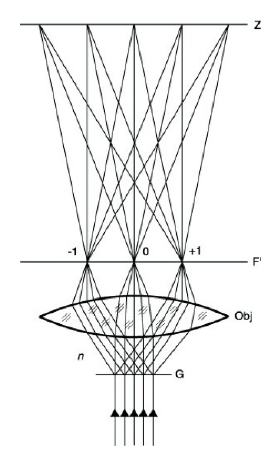
\includegraphics[width=0.3\textwidth]{abes}
	\caption{Konstruktion des primären und sekundären Bildes bei einem Liniengitter; Primärbild bei F, Sekundärbild bei Z} 
\end{figure}
	\item 5. Das abzubildende Objekt sei nun ein Liniengitter. Das Gitter wird mit kohärentem Licht beleuchtet
	(siehe Abb. of.3). Die Gitterspalte stehen dabei senkrecht auf der Zeichenebene. Konstruieren
	Sie primäres sowie sekundäres Bild und skizzieren Sie den Intensitätsverlauf (qualitativ)
	in den entsprechenden Ebenen (Praktikumsheft!). Berücksichtigen Sie bei der Konstruktion
	die Beugungsmaxima 0. sowie +/- 1. Ordnung.\\\\\\\\\\\\\\\\\\\\\\\\\\\\\\\\\\\\\\\\\\\\\\\\ Primäres und sekundäres Bild eines Liniengitters \\\\\\\\\\\\\\\\\\\\\\\\\\
	Intensitätsverlauf in Brenn- und Bildebene

	\item 6. Berechnen Sie den Abstand $\Delta x$ benachbarter Punkte in der hinteren Brennebene von Aufgabe
	Nr. 5\\
	Gesucht werden Orte höchster Intensität, also da, wo es zur größten konstruktiven Interferenz kommt.\\
	$\sin\phi$ =$\dfrac{\lambda}{d}$\\
	Aus Kleinwinkelnäherung folgt: 
	$\sin\phi$ $\approx$ $\tan\phi$ \\
	$\rightarrow \Delta x \approx f \cdot \dfrac{\lambda}{d}$
	
	
	\item 7. Um die Auswirkungen von Eingriffen am primären Bild auf das Endbild beobachten zu können,
	ist es hilfreich, das Endbild (sekundäres Bild) mit dem primären Bild zu vergleichen.
	Dies geschieht am bequemsten, wenn beide Bilder vergrößert nebeneinander auf dem Beobachtungsschirm
	dargestellt werden. Die Problemstellung besteht darin, zwei Bilder, die sich an
	unterschiedlichen Positionen im Strahlengang befinden, in einer Beobachtungsebene (Schirm)
	abzubilden. Dies erreichen Sie mit untenstehendem Aufbau in Abbildung of.4 (nicht maßstabsgetreu,
	alle Maße in mm). Beschriften Sie den Aufbau vollständig und berechnen Sie die Brennweiten
	f1, f2, f4, f5 sowie die Abstände a1,a2,a3 und (a4 + a5). Berücksichtigen Sie bei der
	Wahl der Linsen die Liste der zur Verfügung stehenden Komponenten.\\
	Aus Aufgabe 3 wissen wir: $f_1$= 10 mm und $f_2$= 80mm ergibt $a_1$ = 90 mm, da
	\begin{align*}
a_1 = f_1 + f_2 = 90mm\\
a_2 = f_3 = 200mm\\
\dfrac{1}{f_4}=\dfrac{1}{a_3 + 140mm}+\dfrac{1}{450}\\
\rightarrow f_4 = 200 mm\\
a_3 = 220 mm\\
\dfrac{1}{f_5}=\dfrac{1}{110mm} + \dfrac{1}{a_4+a_5}=\dfrac{1}{100mm}\\
a_4+a_5=1100 mm
	\end{align*}
		\\\\\\\\\\\\\\\\\\\\\\\\\\\\\\\\\\\\\\\
	\item 8. Beschreiben Sie den Charakter der Bilder an den Orten P und Q am Leuchtschirm!\\
	Am Punkt Q kann man das reelle Bild des jeweiligen Objekts beobachten.
	Am Punkt P kann man die scharfen Maxima der Interferenz beobachten.
\item 9. Überlegen Sie sich, wie Sie eine „optische Bank“ (also einen Aufbau mit mehreren optischen
	Komponenten wie z.B. Linsen) justieren sollten. Verdeutlichen Sie sich die Bedeutung einer
	optimalen Ausrichtung der optischen Komponenten auf der optischen Achse anhand Abb. of.5.
	Setzen Sie den Strahlengang des parallel versetzt einfallenden Stahlbündels fort. Was beobachten
	Sie ?\\\\\\\\\\\\\\\\\\\\\\\\\\
	Man muss die Linsenzentren möglichst genau auf der optischen Achse halten. Die errechneten Abstände sollten möglichst genau eingehalten werden. 

	
	Geschieht dies nicht, läuft das Strahlenbündel immer versetzter zur optischen Achse, wodurch keine Abbildung von sauberen Bildern mehr möglich ist.
	
\end{itemize}
\section{Durchführung}
Sie sollen nun den in der Vorbereitung geplanten Aufbau schrittweise realisieren. Bauen Sie dazu die
optischen Komponenten in der Reihenfolge auf, in der sie vom einfallenden Laserbündel durchlaufen
werden. Berücksichtigen Sie außerdem Ihre Überlegungen zur optimalen Justierung einer optischen
Bank.
Nachdem Sie die Anordnung komplett aufgebaut und justiert haben, sollen Sie die Auswirkungen
von Eingriffen (z.B. mit Blenden) im primären Bild am sekundären Bild beobachten. Da das primäre
Bild die Fouriertransformierte des Beugungsobjektes darstellt, entspricht das Ausblenden bestimmter
Details in der Brennebene der abbildenden Linse der Entfernung von einer bzw. mehreren Komponenten
aus dem Fourierspektrum, d.h. bestimmte Raumfrequenzen werden optisch herausgefiltert.
Im Versuch wird gezeigt, wie gezielte Eingriffe in das primäre Bild - also in das Beugungsbild - einerseits
zu einer Verbesserung der Bildqualität beitragen können, andererseits aber auch dazu führen
können, dass zusätzliche, vermeintliche Informationen in das Endbild hineinmanipuliert werden.
\begin{enumerate}
	\item  Bauen Sie die Anordnung gemäß Ihrer Planung bis einschließlich Linse L3 auf. Fügen Sie dann
	als Objekt ein Kreuzgitter an der dafür vorgesehenen Position im Strahlengang ein. Suchen Sie
	mit einem Blatt Papier o.ä. das primäre und sekundäre Bild. Wo befinden sich diese Bilder?
	\item Platzieren Sie nun den Umlenkspiegel am Ende der optischen Bank. Den umgelenkten Strahl
	machen Sie mit Hilfe des Leuchtschirms sichtbar. Nun fügen Sie die Linse L4 möglichst nahe
	zu L3 ein. Verschieben Sie L4 von L3 weg in Richtung Umlenkspiegel. Was beobachten Sie am
	Leuchtschirm?
	\item Bauen Sie nun auch noch die Linse L5 ein und vervollständigen Sie den Aufbau. Wie gehen Sie
	dabei am geschicktesten vor? Skizzieren Sie die Intensitätsverläufe in Ihr Heft!
	\item  Entfernen Sie nun das Kreuzgitter und verwenden Sie einen Doppelspalt als Beugungsobjekt.
	Fügen Sie in der Fokalebene von L3 eine Irisblende ein und blenden Sie nacheinander höhere
	Beugungsordnungen (Raumfrequenzen) aus bis nur noch die 0-te Ordnung die Blende passieren
	kann. Schildern Sie Ihre Beobachtungen. Was folgern Sie daraus für das Auflösungsvermögen
	optischer Geräte?
	\item Wiederholen Sie Aufgabe 4) mit einem Liniengitter als Objekt. Versuchen Sie dann alle ungeraden
	Beugungsordnungen auszublenden. Verwenden Sie dazu die zur Verfügung stehenden
	Mikroskop-Objektträger. Geeignete Blenden lassen sich durch schwarze Striche auf den Objektträgern
	herstellen. Skizzieren und erklären Sie Ihre Beobachtungen.
	\item Verwenden Sie jetzt wieder das Kreuzgitter als Beugungsobjekt. Blenden Sie nun mit einer
	Spaltblende alle horizontalen Beugungsordnungen aus. Was beobachten Sie?
	\item Drehen Sie die Spaltblende um die 0-te Beugungsordnung herum. Zeichnen Sie für geeignete
	Winkel die Intensitätsmuster am Leuchtschirm in ihr Heft und erklären Sie das Zustandekommen
	dieser Muster
	\item Benutzen Sie nun eine Irisblende und finden Sie heraus, welche Beugungsordnungen Sie passieren
	lassen müssen, um das Kreuzgitter vollständig rekonstruieren zu können.
	\item  Verwenden Sie als Objekt den auf Dia belichteten Text. Wie sieht das Beugungsbild aus?
	Versuchen Sie, durch „optische Filterung“ die Bildqualität zu verbessern. Wie erreichen Sie
	dies und woraus besteht die Verbesserung.
	\item Das Objekt sei nun ein Dia, dem eine Punktgitterstruktur überlagert ist. Filtern Sie die
	Gitterstruktur aus dem Endbild heraus. Wie sieht das Bild des Dias aus, nachdem Sie es von
	der Gitterstruktur befreit haben?
\end{enumerate}